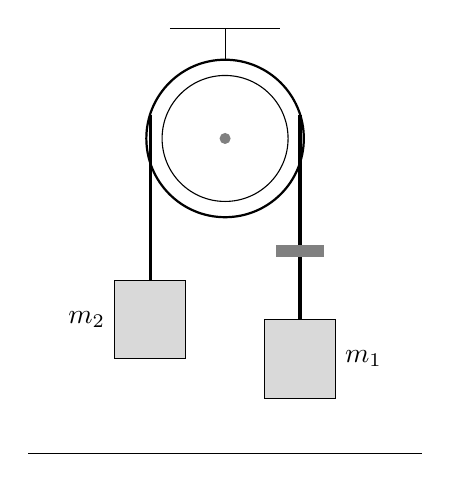
\begin{tikzpicture}
% ceiling
\draw (1.8,5.4) -- (3.2,5.4);
\draw (2.5,5.4) -- (2.5,5);
% pulley
\draw[thick] (2.5,4) circle (1);
\draw (2.5,4) circle (0.8);
\fill[gray] (2.5,4) circle (2pt);
% cords
\draw[very thick] (1.55,4.3) -- (1.55,2.2);
\draw[very thick] (3.45,4.3) -- (3.45,1.7);
% small stop bar
\fill[gray] (3.15,2.5) rectangle (3.75,2.65);
% masses
\fill[gray!30] (1.1,1.2) rectangle (2.0,2.2);
\draw (1.1,1.2) rectangle (2.0,2.2);
\node[left] at (1.1,1.7){$m_2$};
\fill[gray!30] (3.0,0.7) rectangle (3.9,1.7);
\draw (3.0,0.7) rectangle (3.9,1.7);
\node[right] at (3.9,1.2){$m_1$};
% ground
\draw (0,0) -- (5,0);
\end{tikzpicture}
